\begin{task}

Oblicz, jaka część energi sygnału $f(t)=Sa^2\left(\omega_0 \cdot t\right) \cdot cos\left(\omega_0 \cdot t\right)$ przypada na wartości pulsacji 
$\left| \omega \right| < \omega_0$. Wykorzystaj informację, że transformata sygnału $\Lambda(t)$ jest równa $Sa^2\left(\frac{\omega}{2}\right)$.

\begin{equation}
f(t) = Sa^2\left(\omega_0 \cdot t\right) \cdot cos\left(\omega_0 \cdot t\right)
\end{equation}

\begin{equation}
\Lambda(t) \overset{F}{\rightarrow} Sa^2\left(\frac{\omega}{2}\right)
\end{equation}

\begin{equation}
\frac{E_{\left| \omega \right| < \omega_0}}{E} = ?
\end{equation}

Całkowitą energię sygnału można wyznaczyc z twierdzenia Parsevala:
\begin{equation}
\Parseval{F}
\end{equation}

W tym celu musimy wyznaczyc transformatę sygnału $f(t)$.

W jednym z wcześniejszych zadań obliczyliśmy, że transformata Fouriera sygnału $f(t)=Sa^2\left(\omega_0 \cdot t\right) \cdot cos\left(\omega_0 \cdot t\right)$ jest równa $F(\jmath \omega)=\frac{1}{2 } \cdot \left( \frac{\pi}{ \omega_0 } \cdot \Lambda\left( \frac{\omega - \omega_0}{2\cdot \omega_0}\right) + \frac{\pi}{ \omega_0 } \cdot \Lambda\left( \frac{\omega + \omega_0}{2\cdot \omega_0}\right) \right)$.

Narysujmy widmo amplitudowe sygnału $f(t)$, czyli $\left|F(\jmath \omega)\right|$.

\begin{figure}[H]
	\centering
	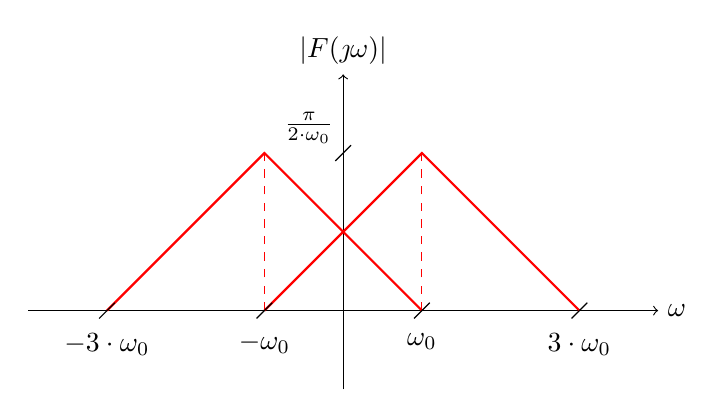
\begin{tikzpicture}
	\draw[->] (-4.0,+0.0) -- (+4.0,+0.0) node[right] {$\omega$};
	\draw[->] (+0.0,-1.0) -- (+0.0,+3.0) node[above] {$\left|F(\jmath \omega)\right|$};
	
	\draw[-,red, thick] (-3.0,0.0) -- (-1.0,+2.0) -- (1.0,0.0);
    \draw[-,red, dashed] (-1.0,+0.0) -- (-1.0,+2.0);
	\draw[-,red, thick] (-1.0,+0.0) -- (1.0,+2.0) -- (3.0,0.0);
    \draw[-,red, dashed] (1.0,+0.0) -- (1.0,+2.0);
	
	\draw[-] (-0.1,+2.0-0.1)--(+0.1,+2.0+0.1) node[midway, above left] {$\frac{\pi}{2 \cdot \omega_0}$};
	
	\draw[-] (-3.0-0.1,-0.1)--(-3.0+0.1,0.1) node[midway, below, outer sep=5pt,align=center] {$-3 \cdot \omega_0$};
	\draw[-] (-1.0-0.1,-0.1)--(-1.0+0.1,0.1) node[midway, below, outer sep=5pt,align=center] {$-\omega_0$};
	\draw[-] (1.0-0.1,-0.1)--(1.0+0.1,0.1) node[midway, below, outer sep=5pt,align=center] {$ \omega_0$};
	\draw[-] (3.0-0.1,-0.1)--(3.0+0.1,0.1) node[midway, below, outer sep=5pt,align=center] {$ 3 \cdot \omega_0$};
	
	\end{tikzpicture}  
\end{figure}

\begin{figure}[H]
	\centering
	\begin{tikzpicture}
	\draw[->] (-4.0,+0.0) -- (+4.0,+0.0) node[right] {$\omega$};
	\draw[->] (+0.0,-1.0) -- (+0.0,+3.0) node[above] {$\left|F(\jmath \omega)\right|$};
	
	\draw[-,red, thick] (-3.0,0.0) -- (-1.0,+2.0) -- (1.0,+2.0) -- (3.0,0.0);
	\draw[-,red, dashed] (-1.0,+0.0) -- (-1.0,+2.0);
	\draw[-,red, dashed] (1.0,+0.0) -- (1.0,+2.0);
	
	\draw[-] (-0.1,+2.0-0.1)--(+0.1,+2.0+0.1) node[midway, above left] {$\frac{\pi}{2 \cdot \omega_0}$};
	
	\draw[-] (-3.0-0.1,-0.1)--(-3.0+0.1,0.1) node[midway, below, outer sep=5pt,align=center] {$-3 \cdot \omega_0$};
	\draw[-] (-1.0-0.1,-0.1)--(-1.0+0.1,0.1) node[midway, below, outer sep=5pt,align=center] {$-\omega_0$};
	\draw[-] (1.0-0.1,-0.1)--(1.0+0.1,0.1) node[midway, below, outer sep=5pt,align=center] {$ \omega_0$};
	\draw[-] (3.0-0.1,-0.1)--(3.0+0.1,0.1) node[midway, below, outer sep=5pt,align=center] {$ 3 \cdot \omega_0$};
	
	\end{tikzpicture}  
\end{figure}

\begin{align*}
\left|F(\jmath \omega)\right| &= \begin{cases}
0 & \omega \in \left( -\infty; -3 \cdot \omega_0 \right> \\
\frac{\pi}{4 \cdot \omega_0^2} \cdot \omega + \frac{3 \cdot \pi}{4 \cdot \omega_0} & \omega \in \left( -3 \cdot \omega_0; -\omega_0 \right> \\
\frac{\pi}{2 \cdot \omega_0} & \omega \in \left(-\omega_0; \omega_0 \right> \\
-\frac{\pi}{4 \cdot \omega_0^2} \cdot \omega + \frac{3 \cdot \pi}{4 \cdot \omega_0} & \omega \in \left(\omega_0; 3 \cdot \omega_0 \right>\\
0 & \omega \in \left(3 \cdot \omega_0; \infty \right)\\
\end{cases}\\
\end{align*}

Podstawiając do wzoru na energię całkowitą, otrzymujemy:
\begin{align*}
E &= \frac{1}{2\pi} \cdot \int_{-\infty}^{\infty} \left|F(\jmath \omega)\right|^2 \cdot d\omega\\
&= \frac{1}{2\pi} \cdot \left[\int_{-\infty}^{-3 \cdot \omega_0} \left|0\right|^2 \cdot d\omega + \int_{-3 \cdot \omega_0}^{-\omega_0} \left|\frac{\pi}{4 \cdot \omega_0^2} \cdot \omega + \frac{3 \cdot \pi}{4 \cdot \omega_0}\right|^2 \cdot d\omega + \int_{-\omega_0}^{\omega_0} \left|\frac{\pi}{2 \cdot \omega_0}\right|^2 \cdot d\omega\right.\\
&\left.+\int_{\omega_0}^{3 \cdot \omega_0} \left|-\frac{\pi}{4 \cdot \omega_0^2} \cdot \omega + \frac{3 \cdot \pi}{4 \cdot \omega_0}\right|^2 \cdot d\omega + \int_{3 \cdot \omega_0}^{\infty} \left|0\right|^2 \cdot d\omega \right]\\
&= \frac{1}{2\pi} \cdot \left[0 + \int_{-3 \cdot \omega_0}^{-\omega_0} \left(\left(\frac{\pi}{4 \cdot \omega_0^2}\right)^2 \cdot \omega^2 + 2 \cdot \frac{\pi}{4 \cdot \omega_0^2} \cdot \frac{3 \cdot \pi}{4 \cdot \omega_0} \cdot \omega + \left(\frac{3 \cdot \pi}{4 \cdot \omega_0}\right)^2\right) \cdot d\omega + \frac{\pi^2}{4 \cdot \omega_0^2}\cdot \int_{-\omega_0}^{\omega_0} d\omega\right.\\
&\left.+ \int_{\omega_0}^{3 \cdot \omega_0} \left(\left(-\frac{\pi}{4 \cdot \omega_0^2}\right)^2 \cdot \omega^2 - 2 \cdot \frac{\pi}{4 \cdot \omega_0^2} \cdot \frac{3 \cdot \pi}{4 \cdot \omega_0} \cdot \omega + \left(\frac{3 \cdot \pi}{4 \cdot \omega_0}\right)^2\right) \cdot d\omega + 0 \right]\\
&= \frac{1}{2\pi} \cdot \left[\frac{\pi^2}{16 \cdot \omega_0^4} \cdot \int_{-3 \cdot \omega_0}^{-\omega_0} \omega^2 \cdot d\omega + \frac{6 \cdot \pi^2}{16 \cdot \omega_0^3} \cdot \int_{-3 \cdot \omega_0}^{-\omega_0} \omega \cdot d\omega + \frac{9 \cdot \pi^2}{16 \cdot \omega_0^2} \cdot \int_{-3 \cdot \omega_0}^{-\omega_0} d\omega + \frac{\pi^2}{4 \cdot \omega_0^2}\cdot \left. \omega\right|_{-\omega_0}^{\omega_0}\right.\\
&\left.+ \frac{\pi^2}{16 \cdot \omega_0^4} \cdot \int_{\omega_0}^{3 \cdot \omega_0} \omega^2 \cdot d\omega - \frac{6 \cdot \pi^2}{16 \cdot \omega_0^3} \cdot \int_{\omega_0}^{3 \cdot \omega_0} \omega \cdot d\omega + \frac{9 \cdot \pi^2}{16 \cdot \omega_0^2} \cdot \int_{\omega_0}^{3 \cdot \omega_0} d\omega \right]\\
&= \frac{1}{2\pi} \cdot \left[\frac{\pi^2}{16 \cdot \omega_0^4} \cdot \left.\frac{\omega^3}{3}\right|_{-3 \cdot \omega_0}^{-\omega_0} 
+ \frac{6 \cdot \pi^2}{16 \cdot \omega_0^3} \cdot \left.\frac{\omega^2}{2}\right|_{-3 \cdot \omega_0}^{-\omega_0} 
+ \frac{9 \cdot \pi^2}{16 \cdot \omega_0^2} \cdot \left.\omega\right|_{-3 \cdot \omega_0}^{-\omega_0} + \frac{\pi^2}{4 \cdot \omega_0^2}\cdot \left(\omega_0-\left(-\omega_0\right)\right)\right.\\
&+\left.\frac{\pi^2}{16 \cdot \omega_0^4} \cdot \left.\frac{\omega^3}{3}\right|_{\omega_0}^{3 \cdot \omega_0} 
- \frac{6 \cdot \pi^2}{16 \cdot \omega_0^3} \cdot \left.\frac{\omega^2}{2}\right|_{\omega_0}^{3 \cdot \omega_0} 
+ \frac{9 \cdot \pi^2}{16 \cdot \omega_0^2} \cdot \left.\omega\right|_{\omega_0}^{3 \cdot \omega_0} \right]\\
&= \frac{1}{2\pi} \cdot \left[\frac{\pi^2}{16 \cdot \omega_0^4} \cdot \left(-\frac{\omega_0^3}{3}-\left(-\frac{27 \cdot \omega_0^3}{3}\right)\right) 
+ \frac{6 \cdot \pi^2}{16 \cdot \omega_0^3} \cdot \left(\frac{\omega_0^2}{2}-\frac{9 \cdot \omega_0^2}{2}\right) 
+ \frac{9 \cdot \pi^2}{16 \cdot \omega_0^2} \cdot \left(-\omega_0-\left(-3 \cdot \omega_0\right)\right)\right.\\
&+\left. \frac{\pi^2}{4 \cdot \omega_0^2}\cdot 2 \cdot \omega_0 + \frac{\pi^2}{16 \cdot \omega_0^4} \cdot \left(\frac{27 \cdot \omega_0^3}{3}-\frac{\omega_0^3}{3}\right) 
- \frac{6 \cdot \pi^2}{16 \cdot \omega_0^3} \cdot \left(\frac{9 \cdot \omega_0^2}{2}-\frac{\omega_0^2}{2}\right) 
+ \frac{9 \cdot \pi^2}{16 \cdot \omega_0^2} \cdot \left(3 \cdot \omega_0 - \omega_0\right) \right]\\
&= \frac{1}{2\pi} \cdot \left[\frac{\pi^2}{16 \cdot \omega_0^4} \cdot \frac{26 \cdot \omega_0^3}{3} 
+ \frac{6 \cdot \pi^2}{16 \cdot \omega_0^3} \cdot \left(-\frac{8 \cdot \omega_0^2}{2}\right) 
+ \frac{9 \cdot \pi^2}{16 \cdot \omega_0^2} \cdot 2 \cdot \omega_0 + \frac{\pi^2}{2 \cdot \omega_0}\right.\\
&+\left. \frac{\pi^2}{16 \cdot \omega_0^4} \cdot \frac{26 \cdot \omega_0^3}{3} 
- \frac{6 \cdot \pi^2}{16 \cdot \omega_0^3} \cdot \frac{8 \cdot \omega_0^2}{2}
+ \frac{9 \cdot \pi^2}{16 \cdot \omega_0^2} \cdot 2 \cdot \omega_0 \right]\\
&= \frac{1}{2\pi} \cdot \left[\frac{26 \cdot \pi^2}{48 \cdot \omega_0} - \frac{48 \cdot \pi^2}{32 \cdot \omega_0}
+ \frac{18 \cdot \pi^2}{16 \cdot \omega_0} + \frac{\pi^2}{2 \cdot \omega_0}+\frac{26 \cdot \pi^2}{48 \cdot \omega_0}
- \frac{48 \cdot \pi^2}{32 \cdot \omega_0} + \frac{18 \cdot \pi^2}{16 \cdot \omega_0}\right]\\
&= \frac{1}{2\pi} \cdot \frac{\pi^2}{2 \cdot \omega_0} \cdot \left[\frac{26}{24} - \frac{48}{16}+ \frac{18}{8} + 1 +\frac{26}{24}
- \frac{48}{16} + \frac{18}{8}\right]\\
&= \frac{\pi}{4 \cdot \omega_0} \cdot \left[\frac{52}{24} - \frac{96}{16}+ \frac{36}{8} + 1\right]\\
&= \frac{\pi}{4 \cdot \omega_0} \cdot \left[\frac{52}{24} - 6 + \frac{108}{24} + 1\right]\\
&= \frac{\pi}{4 \cdot \omega_0} \cdot \left[\frac{160}{24} - 5\right]\\
&= \frac{\pi}{4 \cdot \omega_0} \cdot \left[\frac{160}{24} - \frac{120}{24}\right]\\
&= \frac{\pi}{4 \cdot \omega_0} \cdot \left[\frac{40}{24}\right]\\
&= \frac{5 \cdot \pi}{12 \cdot \omega_0}\\
\end{align*}

Podsumowując, całkowita energia sygnału $f(t) = Sa^2\left(\omega_0 \cdot t\right) \cdot cos\left(\omega_0 \cdot t\right)$ to $E=\frac{5 \cdot \pi}{12 \cdot \omega_0}$.

Energię sygnału dla pewnego zakresu pulsacji, także można wyznaczyc z twierdzenia Parsevala, ale zmieniając granice w całce zgodnie z oczekiwanym zakresem pulsacji, czyli dla pulsacji $\left| \omega \right| < \omega_0$ otrzymamy wzór:
\begin{equation}
 E_{\left| \omega \right| < \omega_0} = \frac{1}{2\pi} \cdot \int_{-\omega_0}^{\omega_0} \left|F(\jmath \omega)\right|^2 \cdot d\omega
\end{equation}

Podstawiając dane dla naszego sygnału otrzymamy:
\begin{align*}
E_{\left| \omega \right| < \omega_0} &= \frac{1}{2\pi} \cdot \int_{-\omega_0}^{\omega_0} \left|F(\jmath \omega)\right|^2 \cdot d\omega\\
&= \frac{1}{2\pi} \cdot \int_{-\omega_0}^{\omega_0} \left|\frac{\pi}{2 \cdot \omega_0}\right|^2 \cdot d\omega\\
&= \frac{1}{2\pi} \cdot \int_{-\omega_0}^{\omega_0} \left(\frac{\pi}{2 \cdot \omega_0}\right)^2 \cdot d\omega\\
&= \frac{1}{2\pi} \cdot \left(\frac{\pi}{2 \cdot \omega_0}\right)^2 \cdot \int_{-\omega_0}^{\omega_0} d\omega\\
&= \frac{1}{2\pi} \cdot \left(\frac{\pi^2}{4 \cdot \omega_0^2}\right) \cdot \left.\omega\right|_{-\omega_0}^{\omega_0}\\
&= \frac{\pi}{8 \cdot \omega_0^2} \cdot (\omega_0 - (-\omega_0))\\
&= \frac{\pi}{8 \cdot \omega_0^2} \cdot (2 \cdot \omega_0)\\
&= \frac{\pi}{4 \cdot \omega_0}\\
\end{align*}

Podsumowując $ E_{\left| \omega \right| < \omega_0} = \frac{\pi}{4 \cdot \omega_0}$.

Teraz możemy obliczyć:
\begin{equation}
\frac{E_{\left| \omega \right| < \omega_0}}{E} = ?
\end{equation}

Podstawiając nasze wczesniejsze wyniki otrzymujemy:
\begin{align*}
\frac{E_{\left| \omega \right| < \omega_0}}{E} = \frac{\frac{\pi}{4 \cdot \omega_0}}{\frac{5 \cdot \pi}{12 \cdot \omega_0}} =\frac{\pi}{4 \cdot \omega_0} \cdot \frac{12 \cdot \omega_0}{5 \cdot \pi} =\frac{12}{20} =\frac{6}{10}=60\%
\end{align*}

Dla pulsacji z zakresu $\left| \omega \right| < \omega_0$ przypada $60\%$ energi sygnału.

\end{task}

